\documentclass[conference]{IEEEtran}
\IEEEoverridecommandlockouts

\usepackage{cite}
\usepackage{amsmath,amssymb,amsfonts}
\usepackage{multicol}
\usepackage{algorithmic}
\usepackage{graphicx}
\usepackage{textcomp}
\usepackage{xcolor}
\usepackage{float}
\usepackage[hidelinks]{hyperref}


\def\BibTeX{{\rm B\kern-.05em{\sc i\kern-.025em b}\kern-.08em T\kern-.1667em\lower.7ex\hbox{E}\kern-.125emX}}

\begin{document}

%===========================
% SMALLER TITLE FONT
\title{\Large
Control and Visualization of an Android-Based Autonomous Navigation System\\
Using Dead Reckoning and SLAM
}


%===========================
% AUTHOR BLOCK (3 UP, 2 DOWN WITH MORE SPACING)
%===========================
% CLEAN AUTHOR BLOCK (NO SYMBOLS + CLICKABLE EMAILS)

\author{%
\begin{tabular}{ccc}
\textbf{Jainil Patel} &
\textbf{Rishi Patel} &
\textbf{Aaryan Sinh Shaurya} \\

\href{mailto:202201030@dau.ac.in}{202201030@dau.ac.in} &
\href{mailto:202201037@dau.ac.in}{202201037@dau.ac.in} &
\href{mailto:202201075@dau.ac.in}{202201075@dau.ac.in} \\
\\
\multicolumn{3}{c}{
\begin{tabular}{cc}
\textbf{Sujal Manavadariya} &
\textbf{Denil Antala} \\

\href{mailto:202201084@dau.ac.in}{202201084@dau.ac.in} &
\href{mailto:202201090@dau.ac.in}{202201090@dau.ac.in}
\end{tabular}
}
\end{tabular}
\thanks{\normalsize \textbf{Control of Autonomous Systems (G18)}}
}



\maketitle

%===========================
\begin{abstract}
Autonomous navigation relies heavily on accurate localization and mapping techniques for real-time control and decision-making. This project presents the design and implementation of an Android-based autonomous navigation system integrating Dead Reckoning (DR) using inertial measurement unit (IMU) sensors and Simultaneous Localization and Mapping (SLAM) using ARCore. The system visualizes real-time trajectories of both DR and SLAM for comparative analysis. A Kalman filter-based estimation framework is explored for minimizing sensor drift. The developed application demonstrates the feasibility of smartphone-based autonomous navigation and provides an experimental platform for analyzing estimation errors, drift behavior, and control accuracy. A video demonstration of the working system is also provided.
\end{abstract}

\begin{IEEEkeywords}
Autonomous Systems, Dead Reckoning, SLAM, ARCore, IMU Sensors, Kalman Filtering, Android Navigation
\end{IEEEkeywords}

%===========================
\section{Introduction}
Autonomous systems require precise estimation of position and orientation in unknown environments to perform navigation and control tasks effectively. Smartphones today contain high-quality inertial sensors and cameras that enable low-cost implementation of navigation algorithms.

Dead Reckoning (DR) estimates position from IMU integration but suffers from drift. SLAM corrects this error using visual features. This project integrates both approaches on Android using ARCore.

%===========================
\section{Problem Statement and Objectives}

\subsection{Problem Statement}
To design and implement a smartphone-based autonomous navigation system capable of estimating and visualizing real-time motion trajectories using DR and SLAM.

\subsection{Objectives}
\begin{itemize}
\item Implement IMU-based Dead Reckoning.
\item Integrate ARCore-based SLAM.
\item Visualize real-time trajectories.
\item Compare drift effects.
\end{itemize}

% %===========================
% \section{Related Work}
% Visual-inertial SLAM systems using ARCore and sensor fusion using Kalman filtering have been widely studied for indoor navigation.

%===========================
\section{System Architecture}
The overall system architecture of the proposed autonomous navigation framework is shown in Figure 1. The system consists of three main modules: Dead Reckoning, SLAM, and Visualization and Control.

The Dead Reckoning module processes inertial data from the smartphone’s accelerometer, gyroscope, and magnetometer. After noise filtering and calibration, the data is integrated to estimate position and orientation without using any GPS or external location services.

In parallel, the SLAM module utilizes the smartphone camera and inertial sensors through the ARCore framework to estimate the six degrees-of-freedom pose using visual feature tracking and mapping.

The outputs of both localization methods are forwarded to a common analysis and visualization layer, where trajectory deviation and drift are evaluated in real time. A session logging module stores motion data for offline analysis and performance evaluation.


\begin{figure}[H]
\centering
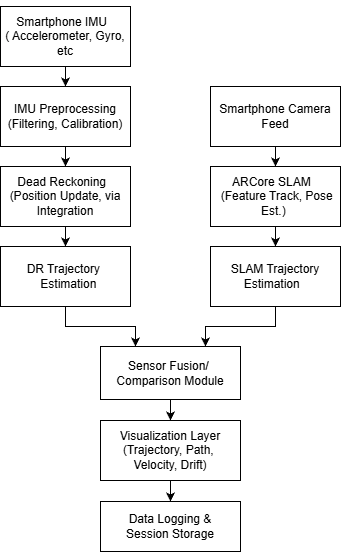
\includegraphics[width=0.8\columnwidth]{system_architecture.png}
\caption{System architecture}
\end{figure}

%===========================
\section{Methodology}

The proposed system estimates the motion of a smartphone-based autonomous platform using two parallel localization techniques: Dead Reckoning (DR) based on inertial sensors and Simultaneous Localization and Mapping (SLAM) using ARCore. The overall methodology consists of sensor data acquisition, preprocessing, motion estimation, trajectory generation, visualization, and performance comparison.

\subsection{System Workflow}

The smartphone collects inertial measurements from the accelerometer, gyroscope, and magnetometer, along with camera frames for SLAM-based pose estimation. The Dead Reckoning and SLAM algorithms operate in parallel, and their estimated trajectories are compared and visualized in real time. Session data is stored for offline analysis. Notably, no GPS or external location services are used in the system.

\subsection{Inertial Sensor Data Acquisition}

The smartphone’s Inertial Measurement Unit (IMU) provides:
\begin{itemize}
\item Linear acceleration: $\mathbf{a}(t) = [a_x, a_y, a_z]^T$
\item Angular velocity: $\boldsymbol{\omega}(t) = [\omega_x, \omega_y, \omega_z]^T$
\item Magnetic field vector: $\mathbf{m}(t) = [m_x, m_y, m_z]^T$
\end{itemize}

These signals are sampled at discrete time intervals $t_k$ and are affected by sensor noise and bias.

\subsection{Preprocessing and Calibration}

To reduce noise and systematic errors, sensor preprocessing is performed before motion estimation. A low-pass filter is applied to accelerometer data to remove high-frequency noise, while gyroscope bias is estimated and compensated. Gravity components are removed using orientation estimates from sensor fusion. This preprocessing ensures improved stability in the Dead Reckoning computations.

\subsection{Dead Reckoning Motion Estimation}

Dead Reckoning estimates the position of the device by integrating acceleration over time. The velocity is computed as:
\begin{equation}
\mathbf{v}_k = \mathbf{v}_{k-1} + \mathbf{a}_k \Delta t
\end{equation}

The position is then updated as:
\begin{equation}
\mathbf{p}_k = \mathbf{p}_{k-1} + \mathbf{v}_k \Delta t
\end{equation}

where $\mathbf{a}_k$, $\mathbf{v}_k$, and $\mathbf{p}_k$ represent the acceleration, velocity, and position at time step $k$, and $\Delta t$ is the sampling period. Since Dead Reckoning relies entirely on inertial integration, errors accumulate over time, resulting in drift.

\subsection{SLAM Using ARCore}

The SLAM module uses the smartphone camera and inertial sensors through ARCore. Visual features are extracted from incoming frames and tracked over time. These features are used to estimate the device pose:
\begin{equation}
\mathbf{x}_k = [x_k, y_k, z_k, \theta_k, \phi_k, \psi_k]^T
\end{equation}

where the vector represents position and orientation in three-dimensional space. ARCore internally performs visual-inertial fusion to correct drift and maintain robust localization even during temporary sensor disturbances.

\subsection{Trajectory Comparison and Visualization}

The DR and SLAM trajectories are projected onto a common 2D coordinate frame for real-time visualization. Separate colored paths are used to distinguish the two motion estimates. Velocity, drift magnitude, and trajectory deviation are displayed on the mobile interface to evaluate the performance difference between the two localization methods.

\subsection{Session Logging and Data Storage}

All estimated positions, velocities, timestamps, and drift values are stored locally during each navigation session. This recorded data is used for offline analysis, result plotting, and system validation.


\subsection{Sensor Fusion Using Kalman Filtering}

To reduce noise and correct drift in the Dead Reckoning estimates, a Kalman filtering approach is studied as part of the sensor fusion process. The Kalman filter combines the inertial predictions from the DR model with corrective pose observations obtained from the SLAM module.

The system state is represented as:
\begin{equation}
\mathbf{x}_k = [x_k, y_k, v_{x_k}, v_{y_k}]^T
\end{equation}

The prediction step is governed by:
\begin{equation}
\mathbf{x}_k^- = \mathbf{A} \mathbf{x}_{k-1} + \mathbf{B} \mathbf{u}_k
\end{equation}

and the measurement update is given by:
\begin{equation}
\mathbf{x}_k = \mathbf{x}_k^- + \mathbf{K}_k (\mathbf{z}_k - \mathbf{H} \mathbf{x}_k^-)
\end{equation}

where $\mathbf{z}_k$ represents the SLAM-based pose measurement and $\mathbf{K}_k$ is the Kalman gain. This fusion improves localization accuracy by balancing fast inertial updates with visually corrected pose information.
\clearpage

%===========================
\section{Implementation}
The proposed system was implemented using Android Studio with native Android APIs and the ARCore SDK. The inertial sensor data was accessed using the Android Sensor Manager, while real-time camera-based tracking was achieved through ARCore. Dead Reckoning computations were performed using processed IMU data, and SLAM-based pose estimates were obtained directly from ARCore. Both trajectories were visualized in real time on a custom Android user interface. The application also supports session data storage for offline analysis.

\begin{figure}[H]
\centering
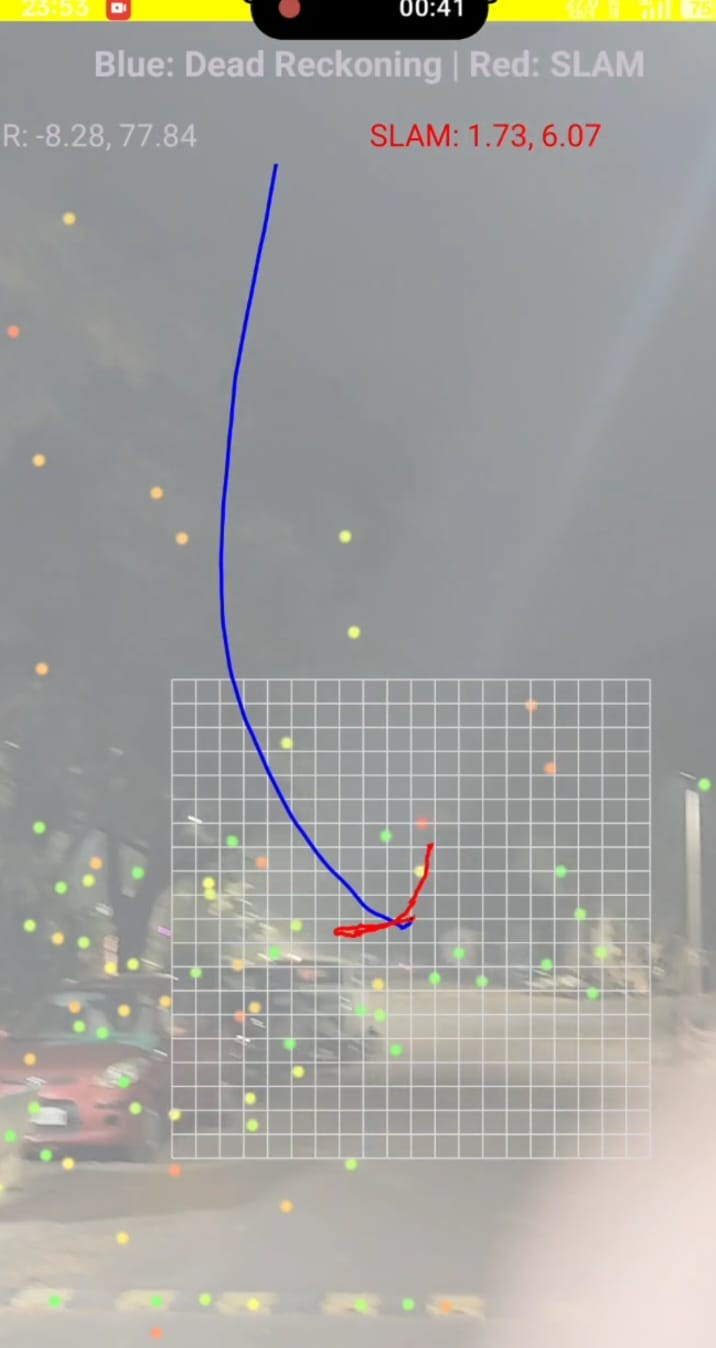
\includegraphics[width=0.8\columnwidth]{ui_placeholder.jpeg}
\caption{Android UI with real-time trajectory}
\end{figure}
\hspace{50em}
%===========================
\\
\\
\\
\\
\\
\\
\\
\section{Results}

The experimental results demonstrate a clear difference between Dead Reckoning (DR) and SLAM-based localization. As observed in the captured trajectories, the DR path (shown in blue) initially follows the motion but gradually deviates due to cumulative integration errors, leading to noticeable drift. In contrast, the SLAM trajectory (shown in red) closely follows the actual motion path with better stability and consistency. The SLAM-based approach benefits from continuous visual feature tracking and pose correction, resulting in significantly reduced drift compared to Dead Reckoning.

\begin{figure}[H]
\centering
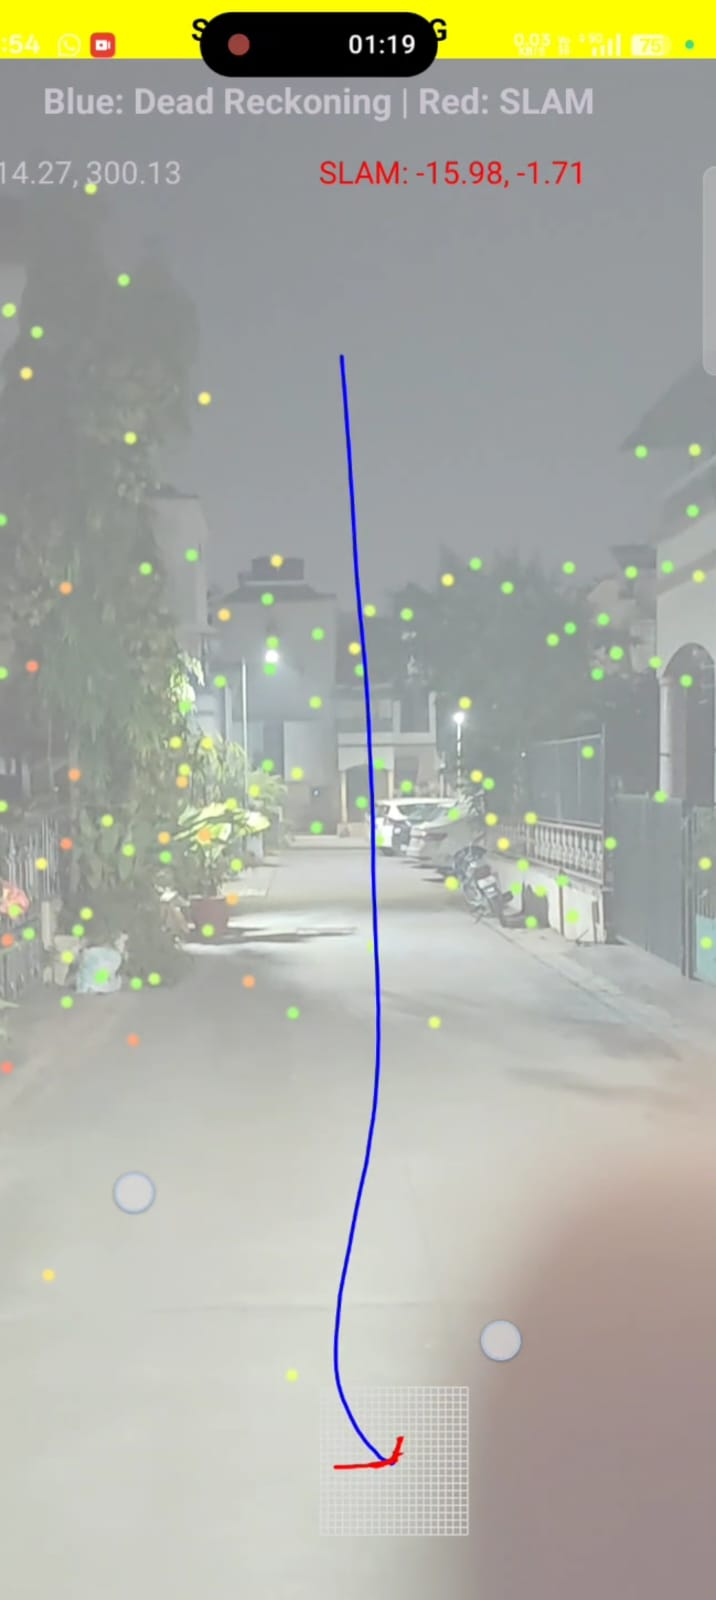
\includegraphics[width=0.85\columnwidth]{cas_dr.jpeg}
\caption{Dead Reckoning trajectory}
\end{figure}

\begin{figure}[H]
\centering
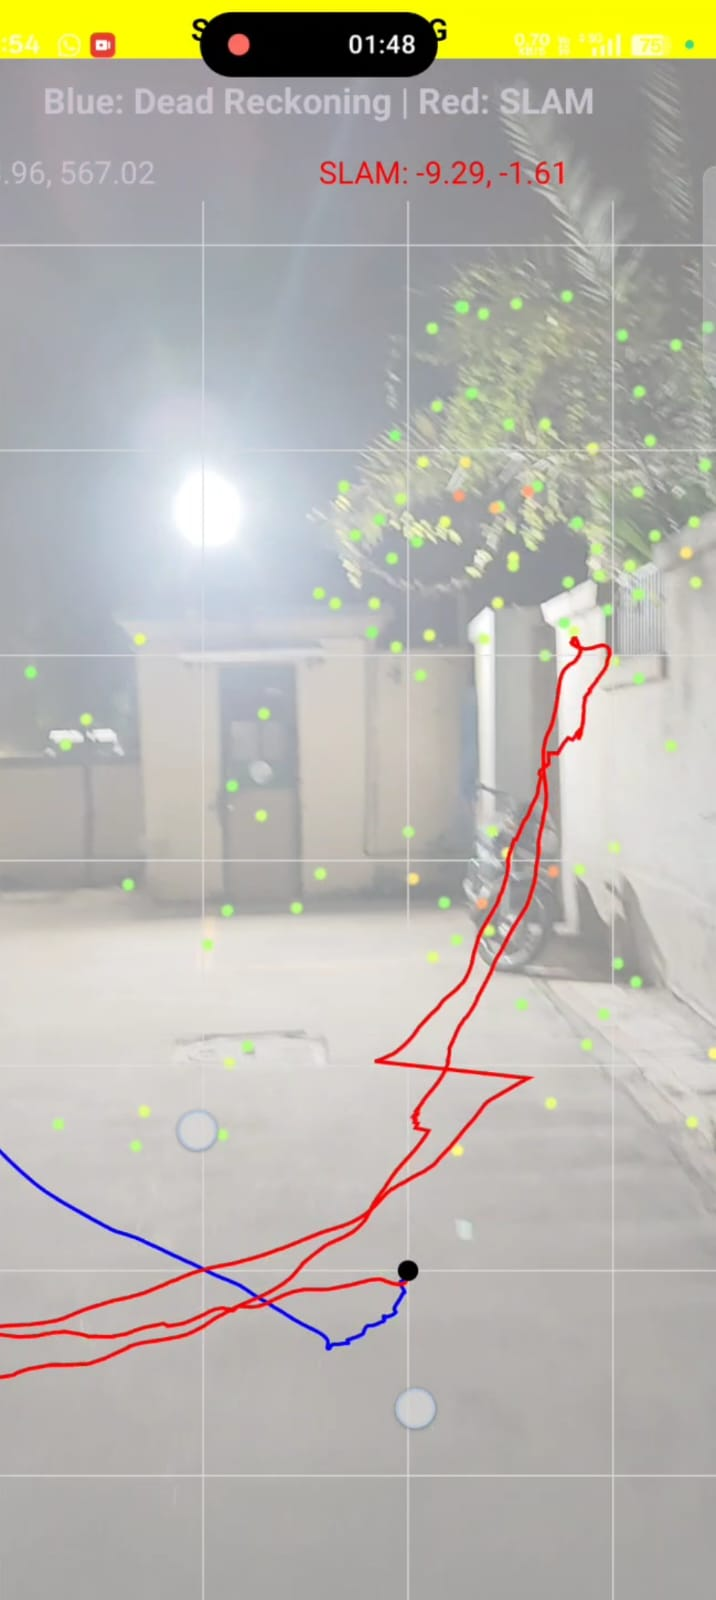
\includegraphics[width=0.85\columnwidth]{cas_slam.jpeg}
\caption{SLAM-based trajectory}
\end{figure}

SLAM provides significantly better stability and lower drift than Dead Reckoning.

\subsection{Video Demonstration}
The working demonstration is available in the submitted project video.

%===========================
\section{Challenges and Limitations}
\begin{itemize}
\item \textbf{Drift in IMU Integration:} The Dead Reckoning method relies on double integration of acceleration data, which leads to cumulative errors over time. Even small sensor biases result in significant positional drift during long motion sequences.
\item \textbf{Hardware Dependency of ARCore:} The performance of the SLAM module is highly dependent on the smartphone’s camera quality, processing power, and sensor accuracy. Older or low-end devices may experience reduced tracking stability and frame drops.
\item \textbf{Sensor Noise and Environmental Disturbances:} Inertial sensors are affected by measurement noise and vibrations, while the SLAM system is sensitive to poor lighting conditions, motion blur, and lack of distinct visual features, which can degrade localization accuracy.
\end{itemize}
%===========================
\section{Deliverables}
\begin{itemize}
\item \textbf{Video Demonstration:} 
\href{https://drive.google.com/file/d/1R3T7pmVKKfZG5sI9E-ViUi_rIJtwWAVJ/view?usp=sharing}{Click here to view}

\item \textbf{Source Code (ZIP File):} 
\href{https://drive.google.com/drive/folders/1zgsUkooMV4mZQ7jU2X09KmtXHL11xYzy?usp=sharing}{Click here to download}
\end{itemize}



%===========================
\section{Future Work}
\begin{itemize}
\item Extended Kalman Filters.
\item Persistent environment mapping.
\item Multi-agent SLAM.
\end{itemize}

%===========================
\section{Conclusion}
The project successfully demonstrates a hybrid autonomous navigation system using Android. SLAM greatly improves localization accuracy over pure Dead Reckoning.

%===========================
\begin{thebibliography}{99}

\bibitem{slam} H. Durrant-Whyte and T. Bailey, ``Simultaneous Localization and Mapping,'' IEEE Robotics and Automation Magazine.

\bibitem{arcore} Google, ``ARCore Developer Documentation.''

\bibitem{imu} D. Titterton and J. Weston, ``Strapdown Inertial Navigation Technology,'' IET.

\end{thebibliography}

\end{document}
